\chapter{Fundamentação Teórica}
\label{cap:fundamentacao-teorica}

Este capítulo apresenta os conceitos necessários para compreender o funcionamento e a avaliação do EDGAR. Inicialmente, a Seção~\ref{sec:llms_e_alucinacoes} aborda os grandes modelos de linguagem e as alucinações no contexto educacional. A Seção~\ref{sec:rag_tradicional} explica a geração aumentada por recuperação (RAG) e suas limitações. A Seção~\ref{sec:busca_semantica} apresenta a busca semântica e os bancos de dados vetoriais. Em seguida, a Seção~\ref{sec:rag_multimodal} discute o processamento multimodal e a granularidade da recuperação. A Seção~\ref{sec:segmentacao_layout} apresenta a análise da estrutura dos documentos e a extração textual. Por fim, a Seção~\ref{sec:engenharia_contexto} aborda a organização das evidências e as métricas utilizadas para avaliar sistemas RAG.

\section{Grandes modelos de linguagem e alucinações no ensino}
\label{sec:llms_e_alucinacoes}

Os grandes modelos de linguagem, ou \textit{Large Language Models} (LLMs), são sistemas de inteligência artificial capazes de interpretar instruções e produzir textos em linguagem natural. Esses modelos resultam de avanços no Processamento de Linguagem Natural (PLN) \citeb{jurafsky2024speech} e passaram a ser utilizados em aplicações como assistentes conversacionais, sumarização de textos e apoio ao aprendizado \citeb{zhao2026survey}.

O funcionamento desses modelos baseia-se em padrões aprendidos durante o treinamento. Ao receber uma pergunta, o LLM considera o contexto fornecido e gera uma resposta progressivamente, prevendo a sequência de unidades de texto, chamadas \textit{tokens} \citeb{tunstall2022natural}. Embora esse processo permita produzir explicações coerentes, a fluidez da resposta não constitui uma verificação de sua veracidade. Sem mecanismos externos de consulta e validação, o modelo pode apresentar informações plausíveis, mas incorretas \citeb{Ji_2023}.

Esse problema é conhecido como alucinação. Na literatura, distinguem-se alucinações intrínsecas, quando a resposta contradiz informações fornecidas como contexto, e extrínsecas, quando apresenta afirmações sem respaldo nas fontes disponíveis \citeb{Ji_2023}. Essas falhas podem decorrer de limitações nos dados de treinamento ou da geração de respostas mesmo quando as evidências são insuficientes \citeb{alansari2026large}.

No ambiente educacional, as alucinações merecem atenção porque estudantes podem utilizar as respostas dos LLMs para compreender conceitos ainda desconhecidos e nem sempre dispõem de conhecimento suficiente para identificar erros apresentados de forma convincente \citeb{kasneci2023chatgpt}. Conforme discutido por \citeonline{holmes2023guidance}, o uso de IA generativa na educação exige uma avaliação crítica dessas ferramentas e de seus resultados. Nesse cenário, torna-se relevante investigar abordagens que forneçam evidências documentais ao modelo e permitam ao usuário consultar as fontes que fundamentam suas respostas, sem presumir que isso elimine completamente as alucinações.

\section{Geração aumentada por recuperação tradicional e suas limitações}
\label{sec:rag_tradicional}

A Geração Aumentada por Recuperação, ou \textit{Retrieval-Augmented Generation} (RAG), combina um mecanismo de busca com um modelo gerador, permitindo que informações externas sejam consultadas no momento de responder a uma pergunta \citeb{NEURIPS2020_6b493230}. Na abordagem textual tradicional, os documentos são convertidos em texto e divididos em fragmentos menores, conhecidos como \textit{chunks}, que são preparados para recuperação \citeb{gao2023retrieval}.

Quando o usuário faz uma pergunta, o sistema procura os fragmentos mais relacionados ao seu conteúdo. Os trechos recuperados são incorporados ao contexto fornecido ao LLM, que os utiliza como apoio para elaborar a resposta. Assim, o modelo não depende apenas do conhecimento adquirido em seu treinamento, embora ainda possa interpretar incorretamente as evidências ou produzir afirmações sem fundamento \citeb{NEURIPS2020_6b493230}.

Essa estratégia funciona especialmente bem quando as informações podem ser representadas em texto contínuo. Em documentos didáticos, porém, o significado também pode depender de tabelas, gráficos, fórmulas e diagramas. A extração textual e a divisão em fragmentos fixos podem separar elementos relacionados \citeb{gao2023retrieval} ou deixar de representar informações presentes em imagens \citeb{faysse2025colpali}, comprometendo o contexto disponível para responder a determinadas perguntas.

\section{Busca semântica e bancos de dados vetoriais}
\label{sec:busca_semantica}

Para que um sistema RAG encontre os trechos mais relacionados a uma pergunta, é preciso comparar significados, e não apenas palavras idênticas. Isso é feito por meio de representações numéricas dos textos e de bancos de dados capazes de armazená-las e consultá-las.

\subsection{Representação semântica e recuperação vetorial}
\label{subsec:embeddings}
\label{subsec:similaridade_vetorial}

Para permitir a busca pelo significado, os conteúdos podem ser convertidos em vetores numéricos chamados \textit{embeddings}. Modelos de representação textual, desenvolvidos a partir de avanços como o BERT \citeb{devlin2019bert}, um modelo de linguagem baseado em redes neurais do tipo \textit{Transformer}, transformam palavras, frases ou trechos em vetores cujas posições refletem relações aprendidas entre os textos. Dessa forma, uma consulta pode recuperar conteúdos semanticamente próximos mesmo quando não utiliza exatamente as mesmas palavras \citeb{DBLP:journals/corr/abs-1908-10084}.

O BGE-M3, apresentado por \citeonline{chen2024bge}, é um exemplo de modelo capaz de representar textos em diferentes idiomas, sendo utilizado em aplicações de recuperação semântica. Essas representações podem ser utilizadas para indexar diferentes tipos de conteúdo textual, incluindo descrições de elementos visuais, permitindo que essas informações também sejam consideradas durante a busca.

Depois de gerar os vetores da pergunta e dos documentos, é necessário compará-los. Uma medida utilizada para isso é a \textbf{similaridade de cosseno}, que considera o ângulo entre dois vetores, e não apenas seus comprimentos. Quando apontam na mesma direção, o ângulo é de $0^\circ$ e a similaridade é igual a $1$. Quando são perpendiculares, o ângulo é de $90^\circ$ e a similaridade é igual a $0$. Se apontam em direções exatamente opostas, o ângulo é de $180^\circ$ e a similaridade é igual a $-1$. Portanto, a medida varia de $-1$ a $1$, e valores maiores indicam maior alinhamento vetorial \citeb{DBLP:journals/corr/abs-1908-10084}.

A Figura~\ref{fig:similaridade_cosseno} apresenta uma representação bidimensional dessa comparação. Na prática, os \textit{embeddings} possuem muitas dimensões, mas o princípio do cálculo permanece o mesmo.

\begin{figure}[H]

\centering

\begin{minipage}{\textwidth}

\caption{Representação geométrica da métrica de similaridade de cosseno.}

\label{fig:similaridade_cosseno}

\vspace{0.2cm}

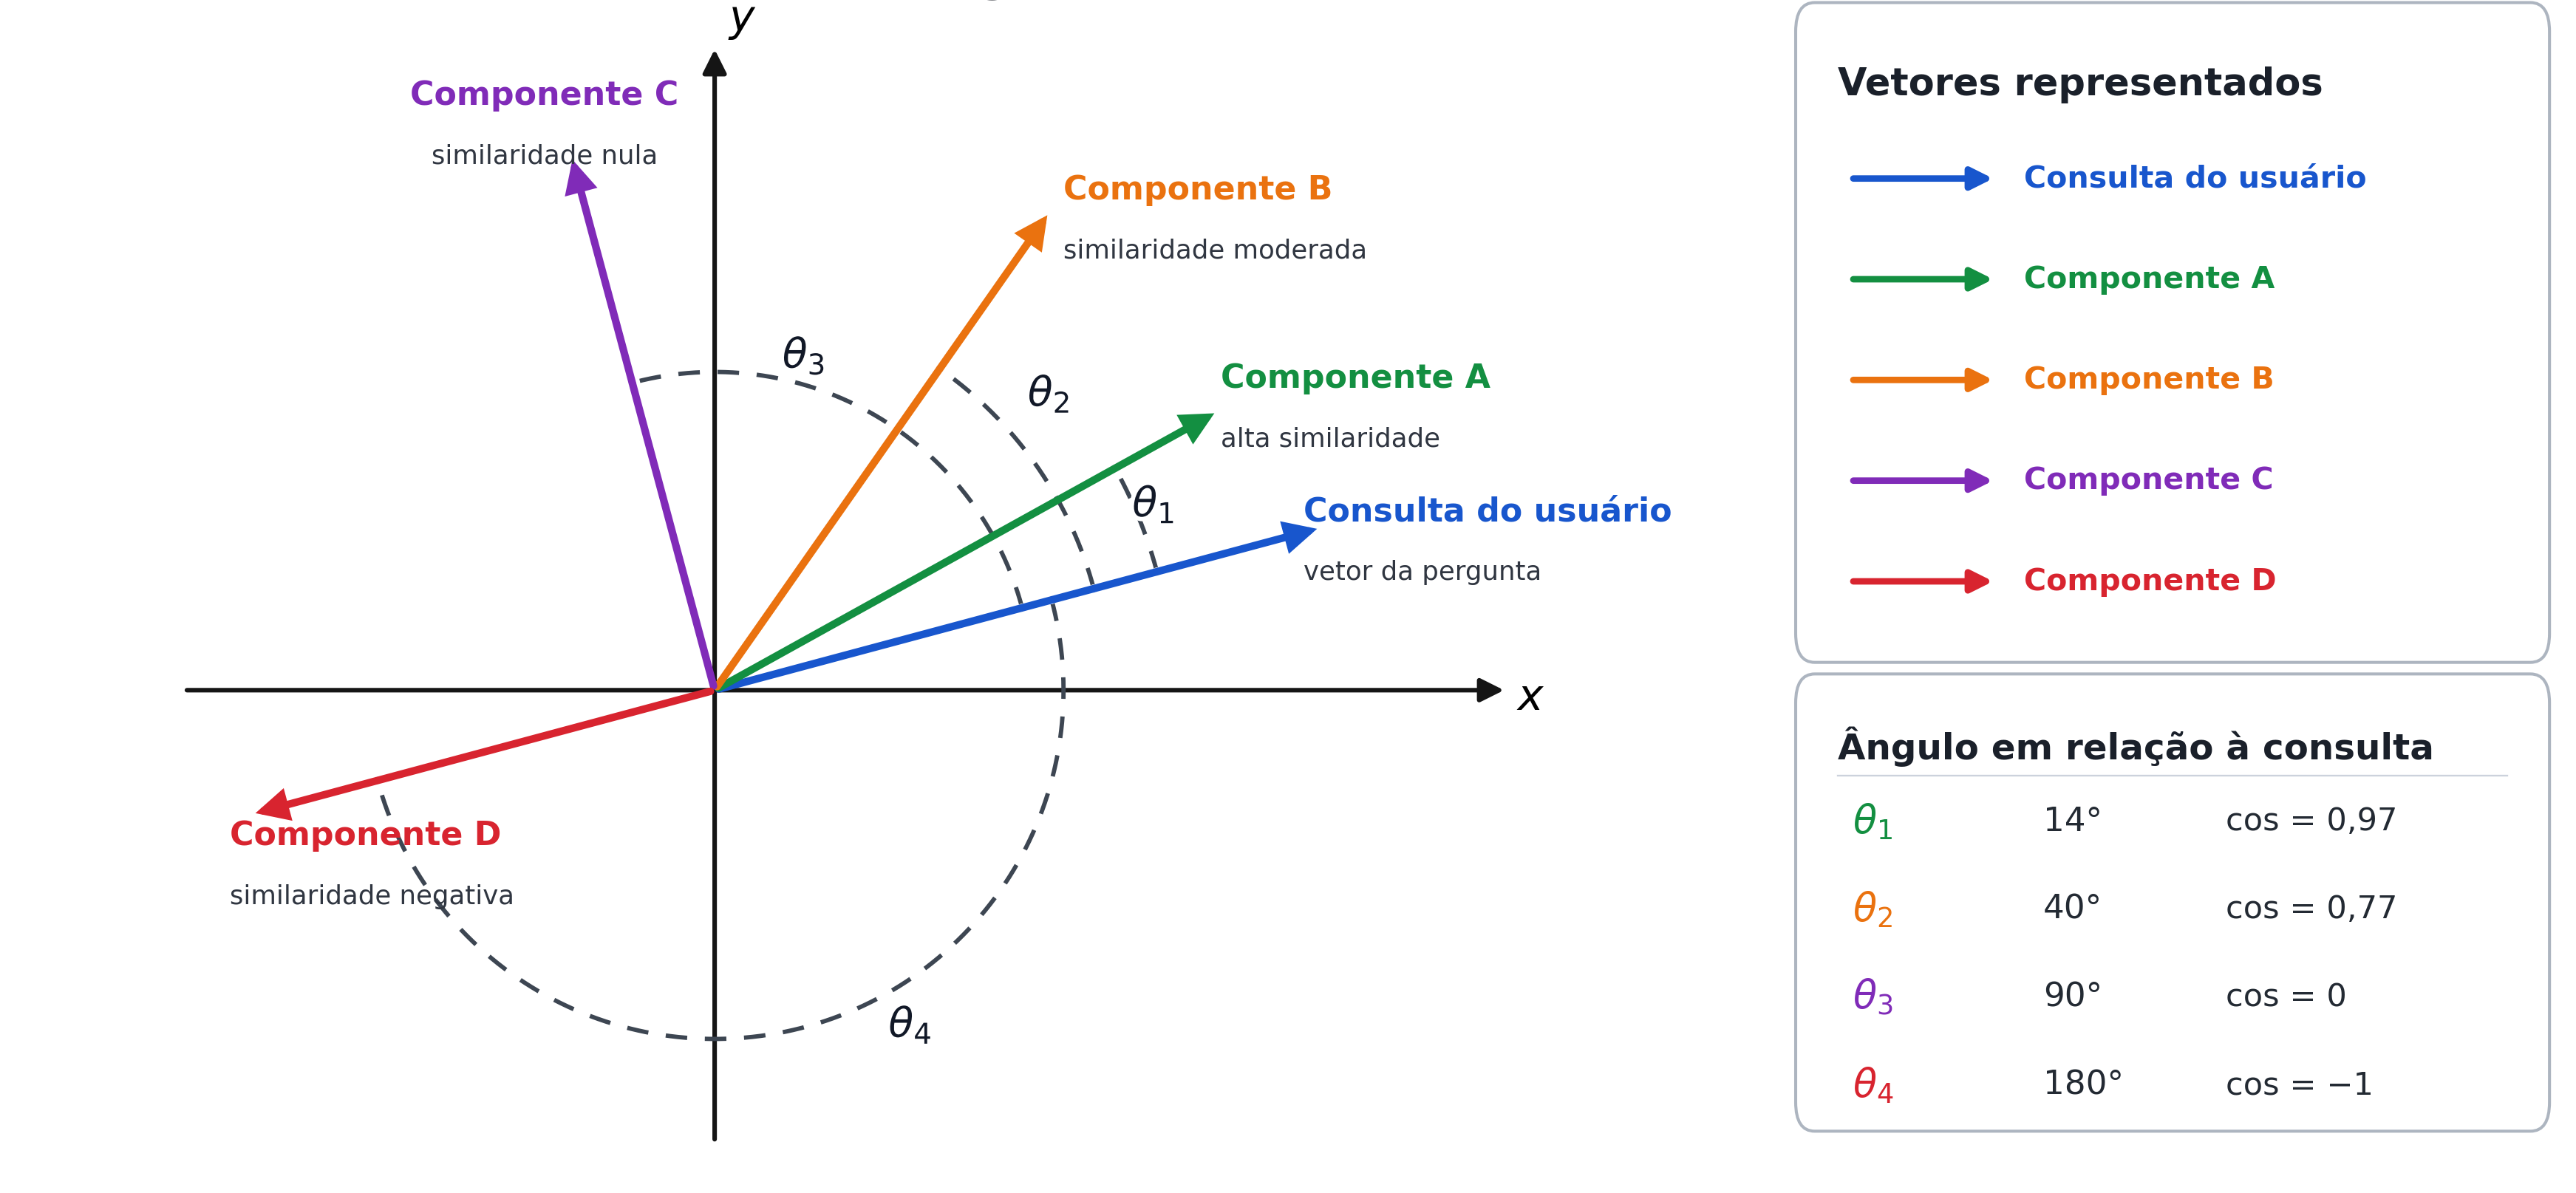
\includegraphics[width=\textwidth]{figuras/similaridade_cosseno}

\vspace{0.1cm}

\par\noindent{\footnotesize Fonte: Elaborado pelo autor.}

\end{minipage}

\end{figure}

\subsection{Bancos de dados vetoriais e metadados}
\label{subsec:bancos_vetoriais}
\label{sec:filtragem_metadados}

Os bancos de dados vetoriais armazenam \textit{embeddings} e permitem recuperar registros por similaridade. Para lidar com grandes conjuntos de vetores, podem utilizar técnicas de busca aproximada por vizinhos mais próximos, conhecidas como \textit{Approximate Nearest Neighbor} (ANN) \citeb{johnson2019billion}. Em sistemas RAG, essa estrutura conecta a pergunta aos conteúdos previamente indexados.

Além dos vetores, os registros podem conter \textbf{metadados}, isto é, informações que descrevem sua origem ou suas características \citeb{gao2023retrieval}. Em documentos PDF, esses atributos podem incluir o identificador do arquivo, o número da página, o tipo do componente e sua localização geométrica. Eles podem apoiar filtros de busca e a apresentação das evidências ao usuário. No presente trabalho, esse vínculo é importante para permitir que componentes recuperados sejam associados às regiões correspondentes do documento original. O uso desses metadados não implica, entretanto, que toda consulta aplique necessariamente um filtro por documento.

\section{Geração aumentada por recuperação multimodal e modelos de visão}
\label{sec:rag_multimodal}

A Geração Aumentada por Recuperação Multimodal (MRAG) amplia o uso do RAG para considerar informações de diferentes modalidades, como texto e imagem \citeb{mei2025survey}. Isso é relevante em materiais didáticos, nos quais uma explicação pode depender de elementos que não são adequadamente representados pela extração textual. Existem diferentes formas de incorporar essas informações: algumas abordagens recuperam representações visuais diretamente, enquanto outras interpretam imagens e utilizam descrições textuais de seu conteúdo na recuperação.

\subsection{Modelos de linguagem e visão}
\label{subsec:vlms_recuperacao}
\label{subsec:vlms_geradores}

Os modelos de linguagem e visão, ou \textit{Vision-Language Models} (VLMs), combinam capacidades de processamento de imagens e linguagem natural \citeb{Yin_2024}. Em determinadas arquiteturas, são empregados para representar visualmente documentos e compará-los com consultas textuais. O ColPali, por exemplo, utiliza representações visuais das páginas para realizar a recuperação sem exigir que todo o seu conteúdo seja previamente convertido em texto \citeb{faysse2025colpali}.

Outra aplicação dos VLMs é a geração de descrições de elementos visuais. Modelos como os da família Qwen-VL podem receber uma imagem acompanhada de uma instrução e produzir um texto sobre seu conteúdo \citeb{bai2023qwen}. Em um documento didático, essa capacidade permite representar em linguagem natural informações de um gráfico ou diagrama e torná-las acessíveis à busca textual. As descrições, porém, podem apresentar omissões ou erros de interpretação, o que influencia a qualidade das evidências disponibilizadas ao sistema.

Essa distinção é importante para compreender o presente trabalho: a arquitetura processa componentes visuais durante a ingestão e incorpora suas descrições aos registros indexados, mas a recuperação vetorial implementada opera sobre representações textuais enriquecidas, e não por comparação direta entre vetores de imagem e texto.

\subsection{Ruído contextual e granularidade de recuperação}
\label{subsec:ruido_contextual}

A granularidade de recuperação corresponde ao tamanho da unidade de informação que um sistema busca e retorna. Em um PDF, essa unidade pode ser uma página inteira, um fragmento textual ou um componente específico, como um parágrafo, uma tabela ou uma figura. Recuperar páginas completas pode fornecer conteúdo útil, mas também incluir informações que não são necessárias para responder à pergunta \citeb{yun2025lilac}.

Esse conteúdo adicional é frequentemente chamado de \textit{ruído contextual}. Estudos sobre o uso de contextos extensos mostram que a presença e a posição de informações relevantes podem afetar o desempenho de modelos de linguagem \citeb{liu2024lost}.
A recuperação em granularidade fina busca oferecer unidades mais localizadas e relacionadas à consulta, evitando depender sempre da página completa. A Figura~\ref{fig:comparativo_ruido} ilustra essa diferença em uma página de livro didático: enquanto o envio da página inteira inclui cabeçalhos, rodapés e parágrafos sobre outros temas, a seleção apenas da tabela pertinente reduz o volume de texto entregue ao modelo gerador. Entretanto, componentes menores também podem perder relações importantes com elementos próximos, comprometendo a compreensão do contexto. Por isso, a escolha da granularidade deve ser avaliada experimentalmente, pois unidades menores não garantem, por si só, melhores resultados de recuperação \citeb{tao2025saki}.

\begin{figure}[H]
\centering
\caption{Comparação ilustrativa entre o envio de uma página inteira e o envio apenas do componente pertinente ao modelo gerador.}
\label{fig:comparativo_ruido}
\vspace{0.2cm}
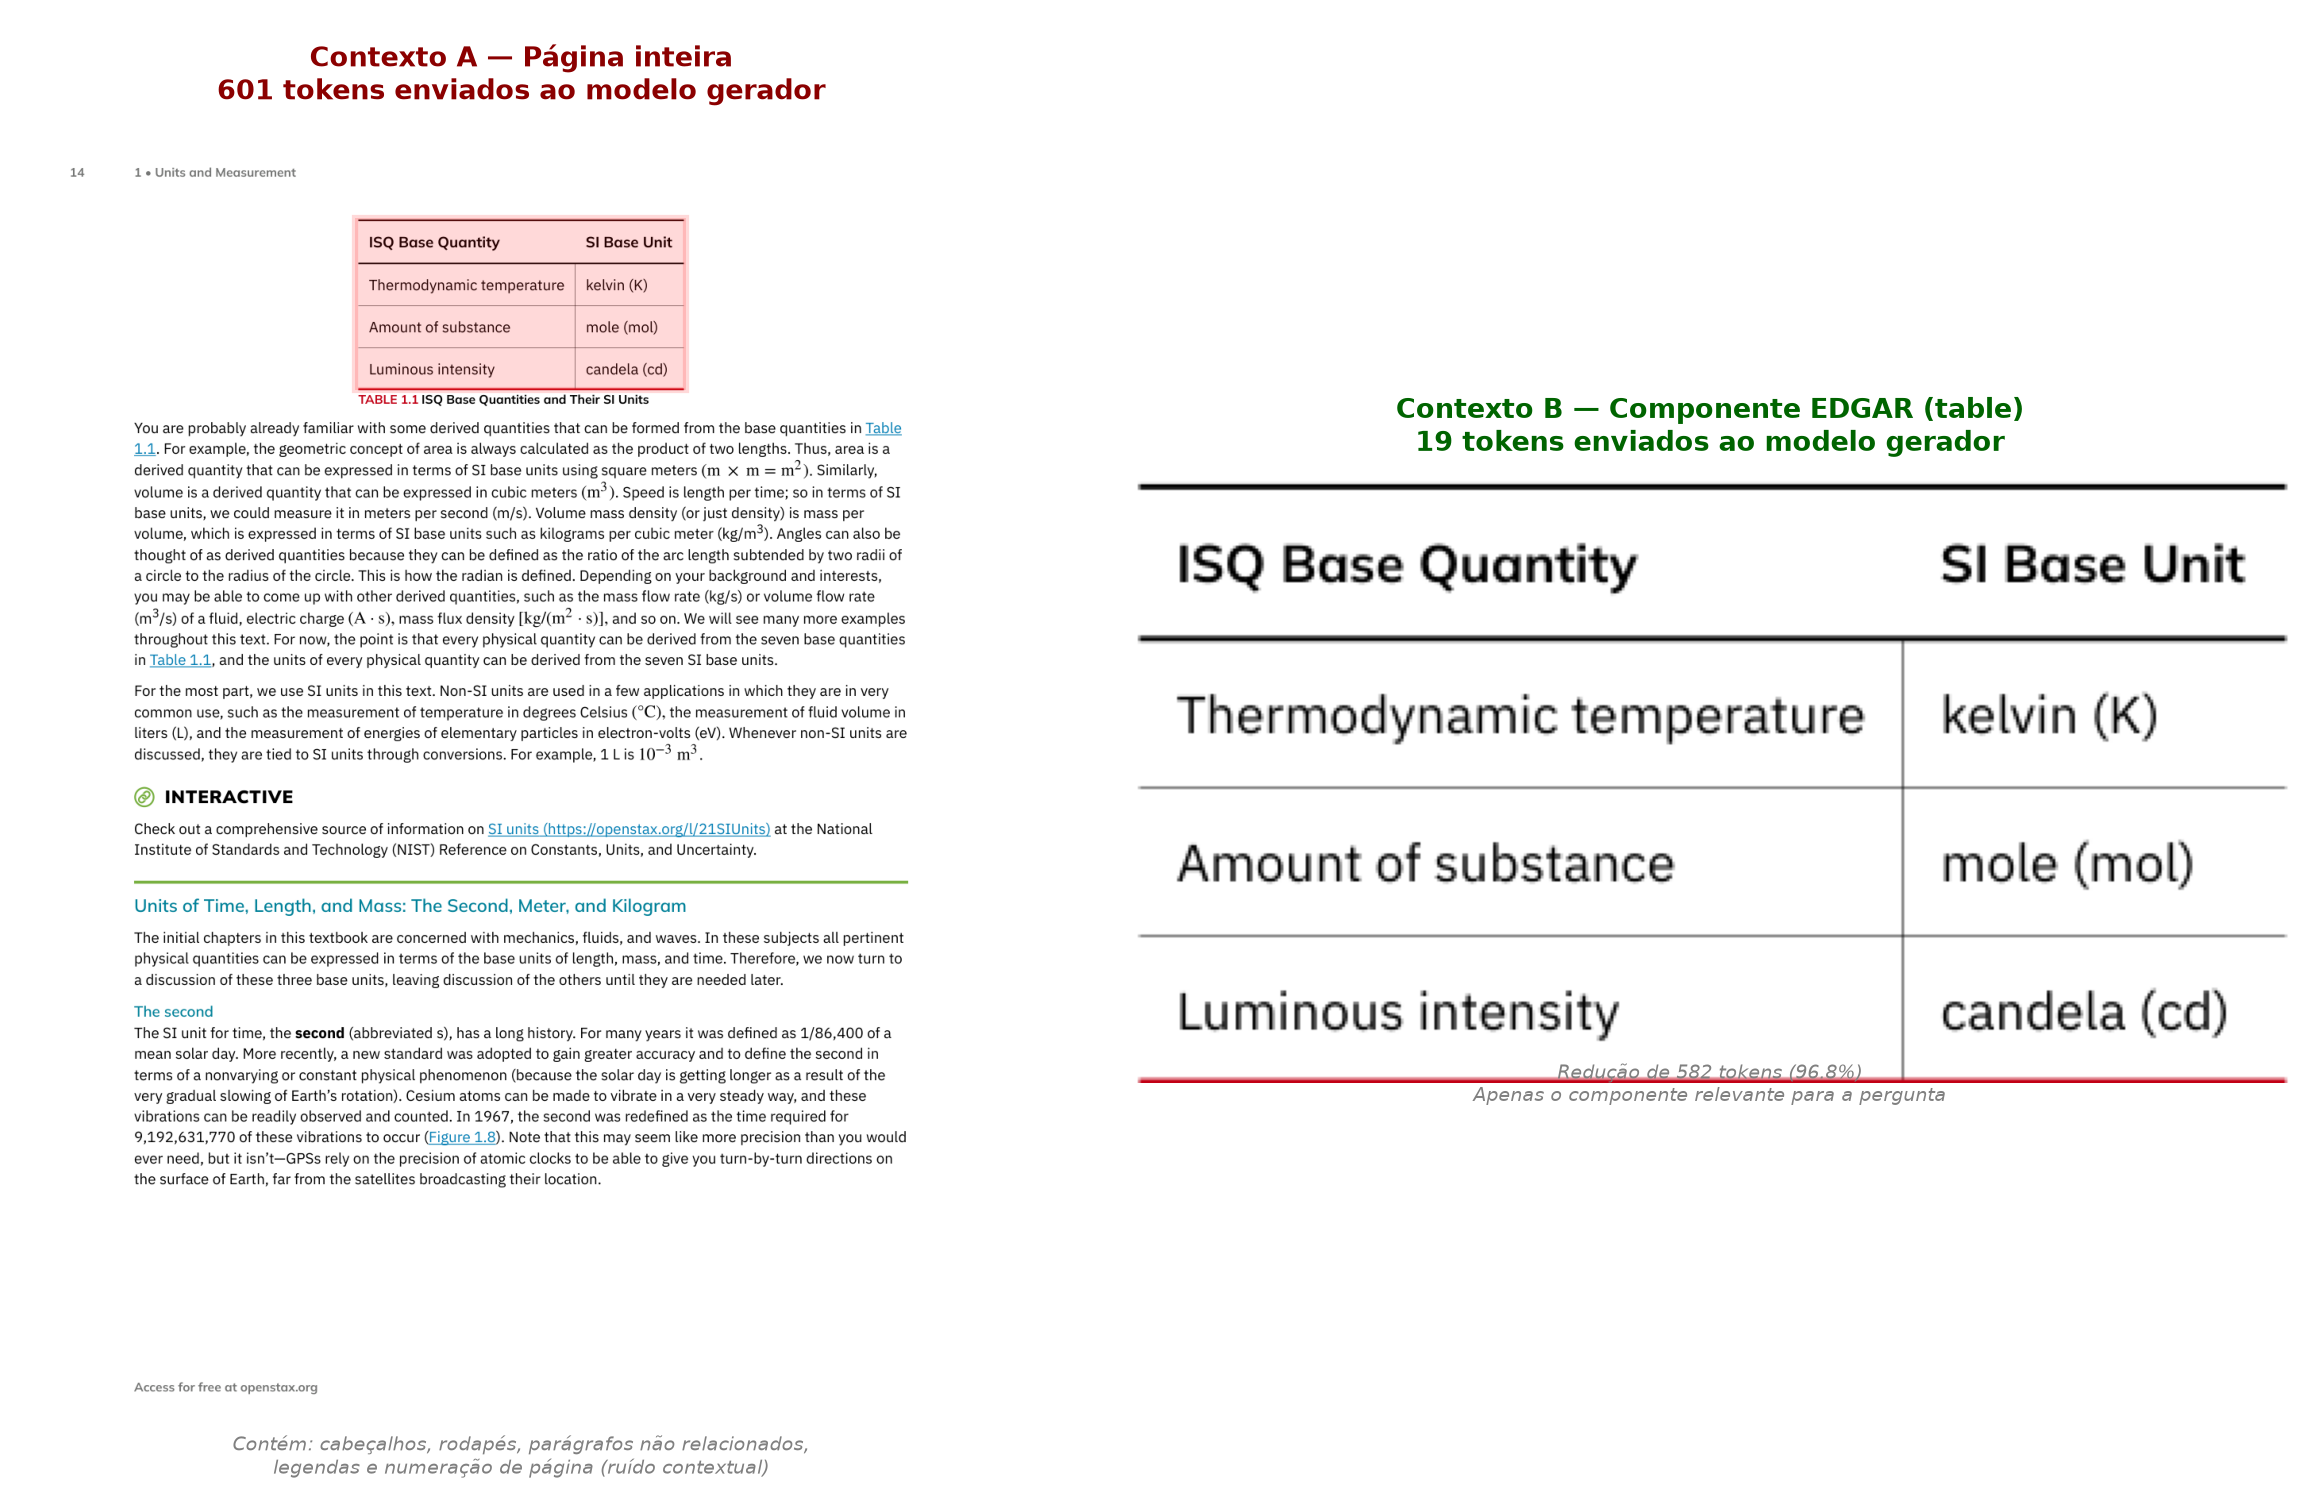
\includegraphics[width=\textwidth]{figuras/comparativo_ruido.png}
\legend{Fonte: Elaborado pelo autor, a partir de \citeonline{moebs2016universityphysics}.}
\end{figure}

\section{Segmentação de layout e processamento de documentos}
\label{sec:segmentacao_layout}

A Análise de Layout de Documentos, ou \textit{Document Layout Analysis} (DLA), reúne técnicas que identificam a organização visual das páginas e delimitam regiões como títulos, parágrafos, tabelas e figuras \citeb{zhong2019publaynet}. Essas regiões costumam ser representadas por caixas delimitadoras (\textit{bounding boxes}), que indicam a posição de cada componente. Essa identificação permite tratar partes do PDF individualmente e estabelecer uma ligação entre seu conteúdo e sua localização no documento.

\subsection{Detecção de componentes documentais}
\label{subsec:yolo_documentos}

Há diferentes abordagens para reconhecer a estrutura de documentos. Modelos da família LayoutLM, por exemplo, exploram informações textuais e espaciais para interpretar a organização das páginas \citebdois{xu2020layoutlm}{huang2022layoutlmv3}. Já modelos de detecção de objetos, inspirados em técnicas como YOLO (\textit{You Only Look Once}), podem identificar regiões a partir da imagem da página \citeb{redmon2016you}. O YOLO é uma família de modelos de visão computacional que localiza objetos em uma imagem em uma única passada.

Entre as abordagens especializadas está o DocLayout-YOLO, desenvolvido para detectar elementos estruturais em documentos \citeb{zhao2024doclayout}. Nesse tipo de processamento, a página é analisada visualmente e o modelo produz regiões correspondentes aos componentes identificados. Essas delimitações podem orientar etapas posteriores de extração textual e descrição visual, embora sua qualidade dependa do desempenho do detector e das características do documento.

\subsection{Extração textual e reconhecimento óptico de caracteres}
\label{subsec:ocr}

Após a identificação das regiões, é necessário obter o conteúdo que será representado e indexado. Em PDFs digitais, parte do texto pode ser extraída diretamente do próprio arquivo. Quando o conteúdo está disponível apenas como imagem, pode ser necessário utilizar Reconhecimento Óptico de Caracteres (OCR), técnica que converte imagens de texto em caracteres pesquisáveis \citeb{smith2007overview}.

A extração localizada utiliza as regiões identificadas pela análise de layout para processar componentes individualmente. Essa estratégia pode ajudar em páginas com colunas, tabelas e diagramas, nas quais a leitura global nem sempre preserva a ordem e a relação entre as informações \citeb{shen2021layoutparser}. Ainda assim, falhas na detecção das regiões ou no reconhecimento de caracteres podem comprometer o texto obtido e, consequentemente, sua recuperação.

\section{Engenharia de contexto em sistemas RAG}
\label{sec:engenharia_contexto}

A engenharia de contexto envolve a seleção e a organização das informações que serão fornecidas ao modelo gerador. Em um sistema RAG, essa etapa define como as evidências recuperadas são apresentadas para apoiar a elaboração da resposta. Seu objetivo é favorecer o uso de informações pertinentes, sem garantir que a resposta produzida esteja correta.

\subsection{Seleção e organização de evidências}
\label{subsec:estrategias_refinamento_contexto}

Nem sempre recuperar mais conteúdo significa oferecer um contexto melhor. Experimentos com tarefas de raciocínio mostram que informações irrelevantes podem prejudicar o desempenho de modelos de linguagem \citeb{shi2023large}. Além disso, a posição das informações relevantes em contextos extensos pode afetar a capacidade dos modelos de utilizá-las \citeb{liu2024lost}. Por isso, sistemas RAG podem selecionar, organizar e identificar as fontes dos fragmentos apresentados ao modelo. No caso de documentos didáticos, a associação entre o conteúdo recuperado e sua localização no PDF também favorece a rastreabilidade, pois permite ao usuário consultar a origem das informações utilizadas na resposta.


\subsection{Métricas de avaliação em sistemas RAG}
\label{subsec:metricas_rag}

A avaliação de sistemas RAG pode considerar separadamente a \textbf{recuperação das evidências} e a \textbf{qualidade das respostas geradas} \citeb{es2024ragas}.

Na recuperação, três medidas são utilizadas neste trabalho. O \textit{Hit@k} verifica se pelo menos uma evidência considerada relevante aparece entre os $k$ primeiros resultados, permitindo avaliar a capacidade do sistema de localizar informações esperadas \citeb{brown2025ragreview}. O \textit{MRR@k} (\textit{Mean Reciprocal Rank}) leva em conta a posição do primeiro acerto: para cada pergunta, atribui o valor $1/r$, em que $r$ é a posição do primeiro resultado correto entre os $k$ primeiros, e $0$ se não houver acerto, e depois calcula a média entre as perguntas. A \textit{Coverage@k} indica em quantas perguntas o resultado esperado aparece entre os $k$ primeiros, com $k$ grande, e mostra se a informação foi alcançada, ainda que em posição distante. Esses princípios podem ser aplicados a diferentes unidades de recuperação, como páginas ou componentes documentais, conforme os critérios definidos em cada avaliação.

Para avaliar a geração, o \textit{framework} RAGAS oferece métricas automatizadas \citeb{es2024ragas}. O Quadro~\ref{quad:metricas_ragas} resume as cinco métricas utilizadas neste trabalho e os nomes em português adotados nas tabelas e nas discussões. Elas são calculadas com o auxílio de um modelo de linguagem que atua como avaliador e julga, por exemplo, se as afirmações da resposta estão de acordo com o contexto ou com a resposta de referência. Por isso, essas medidas dependem de procedimentos automatizados sujeitos a erros e não substituem uma avaliação completa da correção factual ou da adequação das respostas \citeb{saadfalcon2024ares}.

\begin{quadro}[H]
\centering
\caption{Métricas do RAGAS utilizadas e nomes adotados neste trabalho.}
\label{quad:metricas_ragas}
\begingroup
\small
\renewcommand{\arraystretch}{1.2}
\begin{tabularx}{\textwidth}{|p{3.2cm}|p{3.2cm}|X|}
\hline
\textbf{Nome neste trabalho} & \textbf{Nome no RAGAS} & \textbf{O que mede} \\
\hline
Apoio na evidência & \textit{Faithfulness} & Proporção das afirmações da resposta que encontram suporte no contexto fornecido ao gerador. \\
\hline
Pertinência da resposta & \textit{Answer Relevancy} & Quão diretamente a resposta trata da pergunta apresentada. \\
\hline
Correção factual & \textit{Factual Correctness} & Concordância das afirmações da resposta com a resposta de referência escrita pelo autor. \\
\hline
Precisão do contexto & \textit{Context Precision} & Se as evidências relevantes aparecem nas primeiras posições do contexto recuperado. \\
\hline
Cobertura do contexto & \textit{Context Recall} & Se as informações da resposta de referência estão presentes no contexto recuperado. \\
\hline
\end{tabularx}
\endgroup
\legend{Fonte: Elaborado pelo autor, com base na documentação do RAGAS.}
\end{quadro}

Além da recuperação e da geração, a avaliação de sistemas RAG pode considerar aspectos de desempenho, como o tempo necessário para produzir respostas \citeb{brown2025ragreview}. A interpretação dessas medidas depende das etapas efetivamente consideradas, sendo importante distinguir o tempo de geração da latência completa do sistema.
